\chapter{Background}
\label{background}

\section{Introduction}

There are a number of components needed to build the architecture of a web application. The nature of these components is explored below, and their contribution to the creation of a web application is analysed. A more detailed breakdown on their usage within the application is explored in subsequent chapters.

\section{Support for Quality Attributes}

Within the scope of this application, there were a number of quality attributes that were examined. A quality attribute is "part of an applications non-functional requirements, which capture the many facets of \textit{how} the functional requirements of an application are achieved" \parencite{gorton2006essential}. They can related to system design, or may be specific to run time or user centric issues.


\begin{itemize}
\item Security
\begin{itemize}
\item This is the capability of the system to prevent actions that are outside the designed usage, or actions that are malicious in origin. Within an application, "security boils down to understanding the precise security requirements for an application, and devising mechanisms to support them" \parencite{gorton2006essential}.
\end{itemize}
\item Performance
\begin{itemize}
\item This is the capability of the system to respond to actions performed on it within a reasonable time frame. It "defines a metric that states the amount of work an application must perform in a given time" \parencite{gorton2006essential}.
\end{itemize}
\item Usability
\begin{itemize}
\item This is the capability of the system to cater to the requirements of the user, and the how intuitive the system is to use.
\end{itemize}
\item Extensibility
\begin{itemize}
\item This is the capability of the system to cater for future requirements. It is a "measure of how easy it may be to change an application to cater for new functional and non-functional requirements" \parencite{gorton2006essential}
\end{itemize}
\item Productivity
\begin{itemize}
\item This is the influence that the architectural choices of the system affects developer productivity, which has an effect on other quality attributes.
\end{itemize}
\end{itemize}
\begin{table}[H]
\caption{Quality Attributes}
\label{fig:qualityAttributes}
\end{table}

\section{Technologies}

\subsection{Web Application Framework}
The Web Application Framework [WAF] chosen for this project is Spring MVC. Shan and Hua define a WAF as “a defined support structure in which other software applications can be organized and developed” \parencite{shan2006taxonomy}. MVC, or Model-View-Controller, is a software pattern that facilitates the use of a user interface, shown in its classic form in Figure~\ref{fig:mvcclassic}. The intention of this pattern is to form a clear division between domain objects and presentation objects. The Model manages the behaviour and data of the application. The View manages the information obtained from the model and displays it to the user. The Controller manages user input, such as key strokes, mouse movements or a touch display, and can interact and invoke functionality within the Model and/or View.

\begin{figure}[H]
\begin{center}
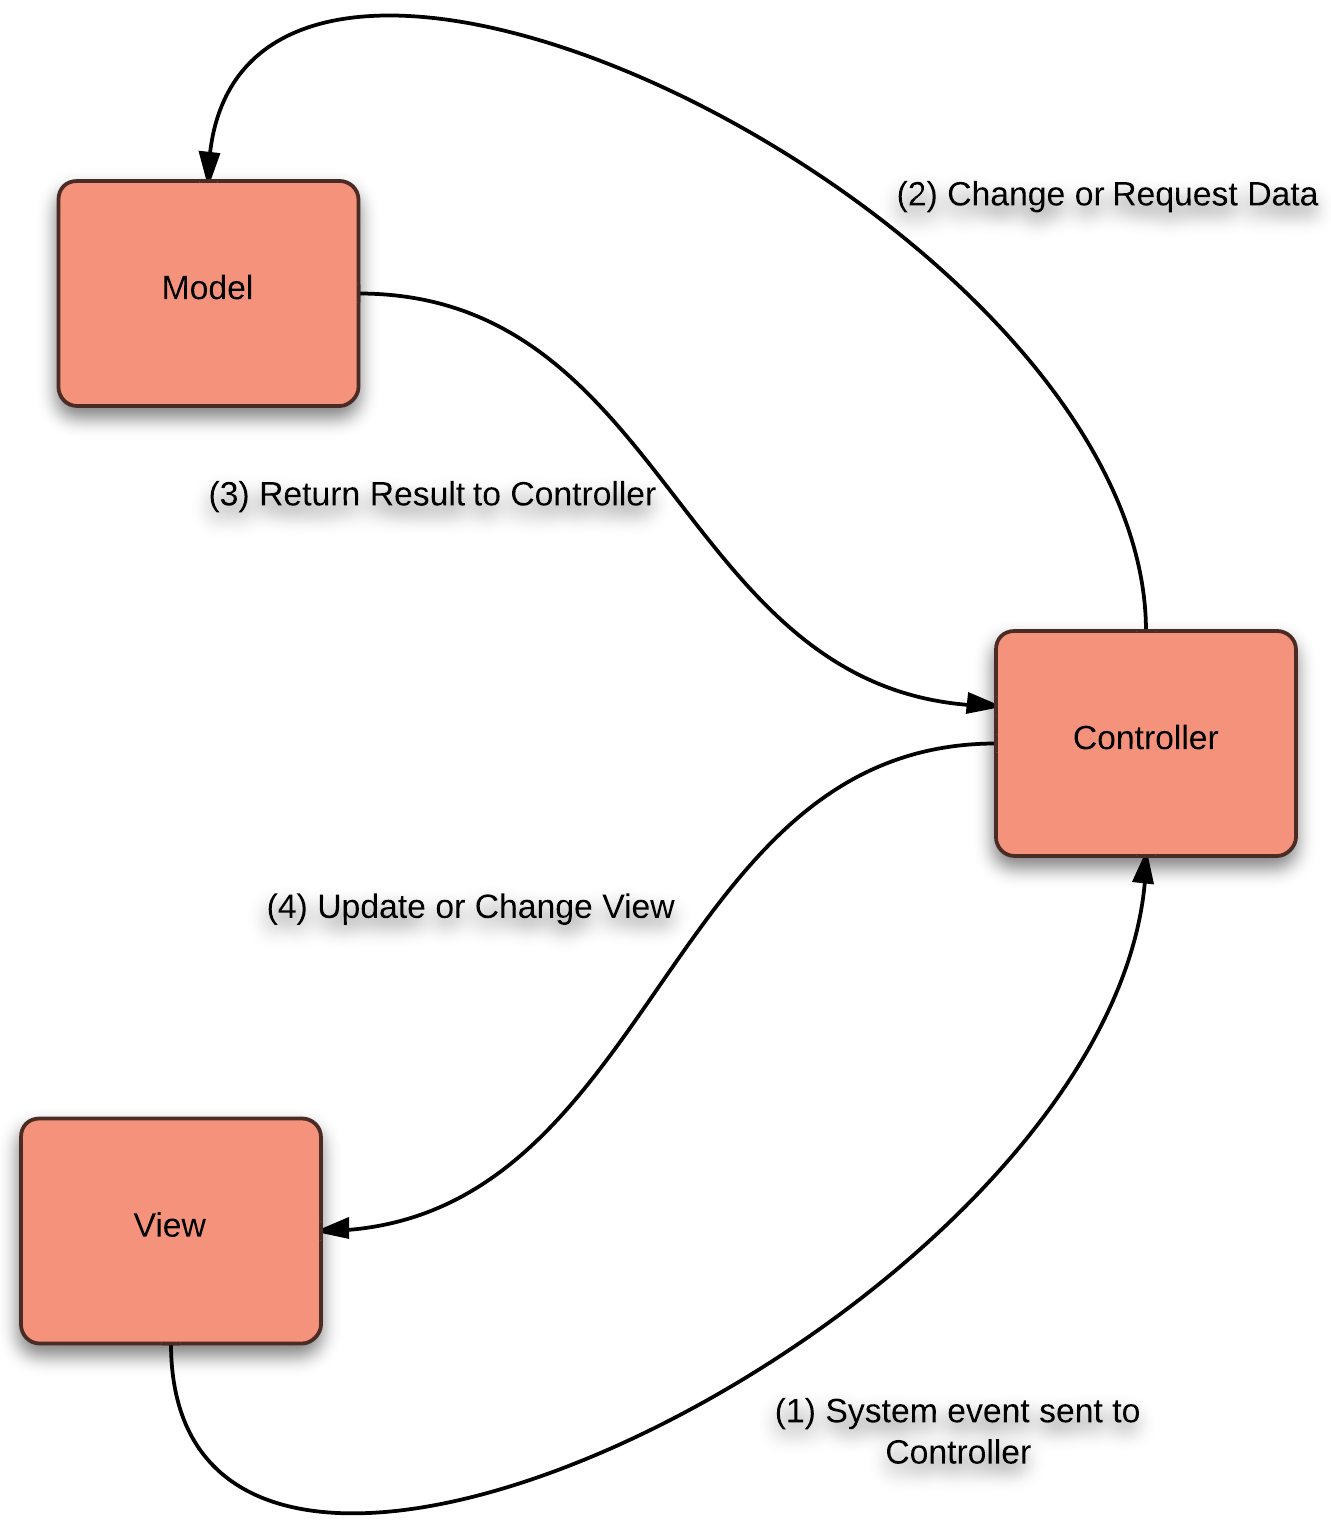
\includegraphics[width=9cm]{mvcclassic.png}
\end{center}
\caption{Classic MVC}
\label{fig:mvcclassic}
\end{figure}

Spring MVC has a \textit{DispatcherServlet}. This is defined within the \textit{web.xml} file, shown in Figure ~\ref{fig:webxml}. This file is located in the WEB-INF folder. Its purpose is to load the application context from a servlet file, defined within this application as \textit{member-servlet.xml}. An Application Context is an interface within the framework. This interface provides the configuration for the application. 

Spring MVC provides a clear separation of roles. Each role, such as a View, Controller, Mapper, Validator, Model and View Resolver, can be encapsulated within a relevant object. It is a request driven framework designed around the \textit{DispatcherServlet}. 

\begin{figure}[H]
\begin{center}
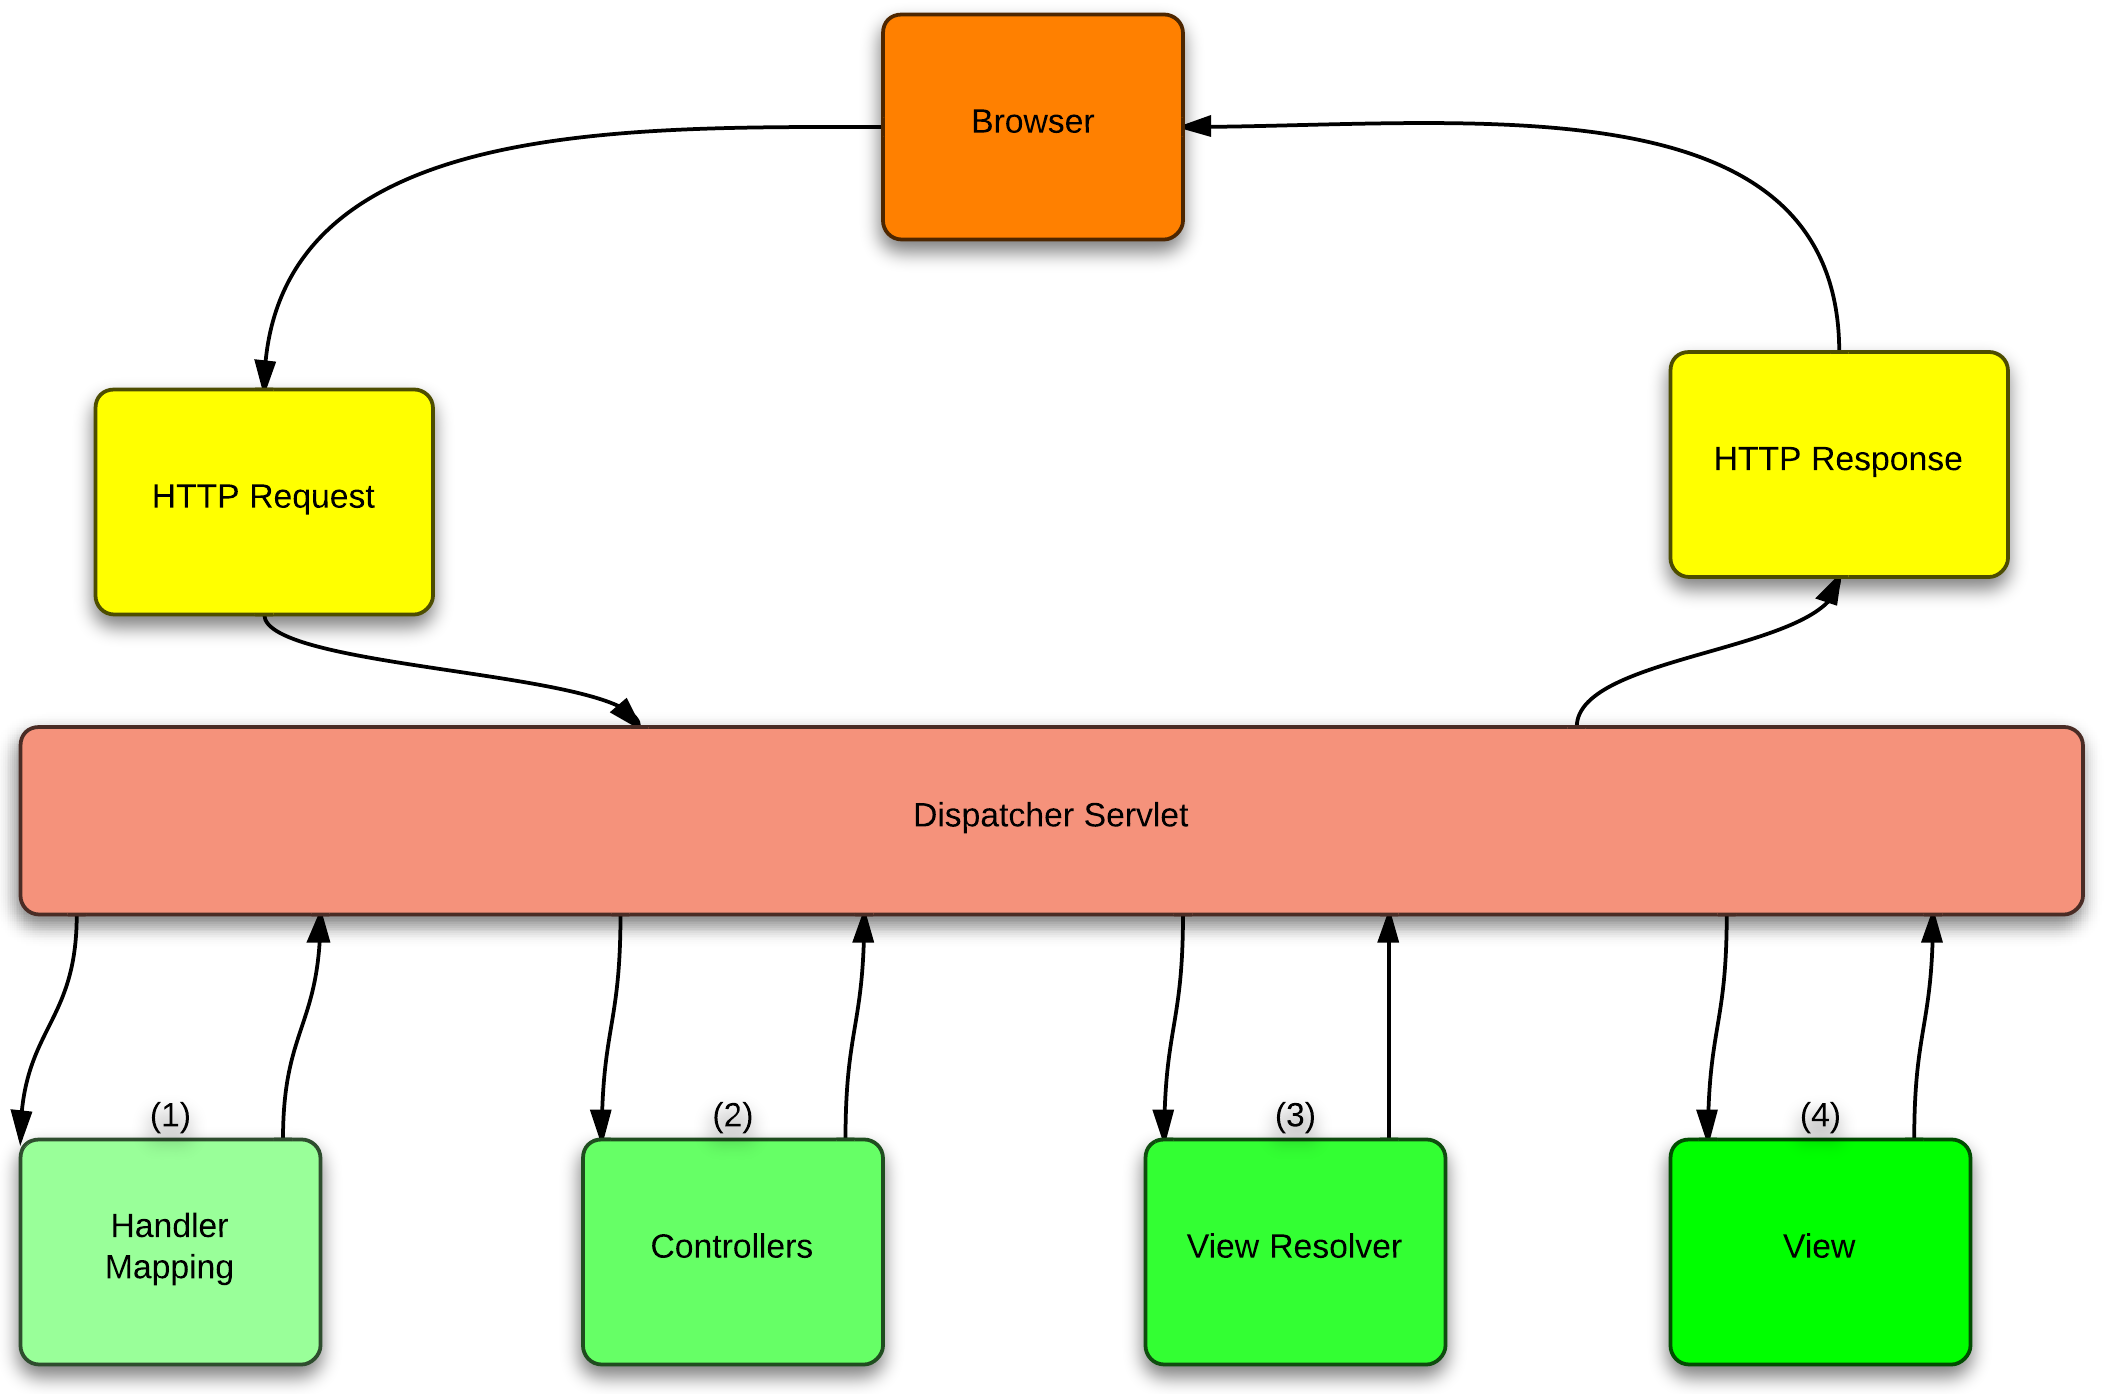
\includegraphics[width=14cm]{dispatchservlet.png}
\end{center}
\caption{DispatcherServlet}
\label{fig:dispatcherflow}
\end{figure}

The \textit{DispatcherServlet} is responsible for handling HTTP requests from the browser. Once it receives these requests, it consults the HandlerMapper, which calls the appropriate Controller. A HandlerMapper takes a value, such as "/admin", and checks which controller handles this mapping. The Controller will take this request, and call the appropriate method, or methods, and interact with the Service layer of the application, if necessary. The View name is then returned to the \textit{DispatcherServlet}, which in turn passes the value to the ViewResolver. 

A ViewResolver provides a mapping between a \textit{view name} and the \textit{view}, that is to say, the web page requested. Once this view is finalised, the \textit{DispatcherServlet} passed any model created within the Controller to the View, which is then rendered by the browser. This process is shown in Figure ~\ref{fig:dispatcherflow}


\begin{lstlisting}
<web-app 
xmlns:xsi="http://www.w3.org/2001/XMLSchema-instance" 
xmlns="http://java.sun.com/xml/ns/javaee" 
xsi:schemaLocation="http://java.sun.com/xml/ns/javaee http://java.sun.com/xml/ns/javaee/web-app_2_5.xsd" 
version="2.5">
  <display-name>monaleen-tennis</display-name>
  <welcome-file-list>
    <welcome-file>index.jsp</welcome-file>
  </welcome-file-list>
  <servlet>
    <description></description>
    <display-name>members</display-name>
    <servlet-name>members</servlet-name>
    <servlet-class>org.springframework.web.servlet.DispatcherServlet</servlet-class>
    <load-on-startup>1</load-on-startup>
  </servlet>
  <servlet-mapping>
    <servlet-name>members</servlet-name>
    <url-pattern>/</url-pattern>
  </servlet-mapping>
  <description>Database</description>
  <resource-ref>
    <description>DB Connection</description>
    <res-ref-name>jdbc/mtc</res-ref-name>
    <res-type>javax.sql.DataSource</res-type>
    <res-auth>Container</res-auth>
  </resource-ref>
  <context-param>
    <param-name>contextConfigLocation</param-name>
    <param-value>
	classpath:beans/dao-context.xml
	classpath:beans/service-context.xml
	classpath:beans/security-context.xml
	</param-value>
  </context-param>
</web-app>
\end{lstlisting}
\begin{figure}[H]
\caption{Spring DispatcherServlet Configuration}
\label{fig:webxml}
\end{figure}

Figure ~\ref{fig:webxml} is the configuration file needed for the \textit{DispatcherServlet}. The file has a number of responsibilities within the application.

\begin{table}[H]
\caption{DispatcherServlet Code}
\begin{itemize}
\item Define DispatcherServlet
\begin{itemize}
\item Line 9: This defines what class the DispatcherServlet implements.
\begin{lstlisting}
 <servlet-class>org.springframework.web.servlet.DispatcherServlet</servlet-class>
\end{lstlisting}
\end{itemize}
\item Define ApplicationContext
\begin{itemize}
\item Line 17-19: This specifies the file that defines the application context of the application
\begin{lstlisting}
<servlet-mapping>
<servlet-name>members</servlet-name>
<url-pattern>/</url-pattern>
 </servlet-mapping>
\end{lstlisting}
\end{itemize}
\item Define DataSource
\begin{itemize}
\item Lines 22-27: This defines the reference to the database, and the DataSource class
\begin{lstlisting}
<resource-ref>
<description>DB Connection</description>
<res-ref-name>jdbc/mtc</res-ref-name>
<res-type>javax.sql.DataSource</res-type>
<res-auth>Container</res-auth>
</resource-ref>
\end{lstlisting}
\end{itemize}
\item Define Context Config Location
\begin{itemize}
\item Lines 28-35: This defines the files that contain the configuration for the DAO, Service and Security context files.
\begin{lstlisting}
<context-param>
<param-name>contextConfigLocation</param-name>
<param-value>
classpath:beans/dao-context.xml
classpath:beans/service-context.xml
classpath:beans/security-context.xml
</param-value>
</context-param>
\end{lstlisting}
\end{itemize}
\end{itemize}
\label{fig:webxmlExplain}
\end{table}

The \textit{Controller}, within the Spring MVC framework, is designed for preparing a model with data, and selecting a view which will represent that data. This is done through the use of a \textit{RequestMapping} annotation, which is discussed in further detail in Section~\ref{sec:impl} of this report.

The default \textit{ViewResolver} within the Spring MVC is the InteralResourceViewResolver, depicted in Figure ~\ref{fig:defaultViewRes}. This is defined with the \textit{members-servlet.xml} file in the application, which is the structure of the \textit{DispatcherServlet}. This class takes the value that is returned by a Controller, and passes a View to the DispatcherServlet. The browser can then render this view. It is important that any views, such as JSP files within the scope of this application, are stored within the \textit{WEB-INF} folder. This is to ensure that the files are treated as an internal resource, and as such, are only accessible by the servlet, or the Controller classes within the application.

\begin{lstlisting}
<bean id="jspViewResolver"
	class="org.springframework.web.servlet.view.InternalResourceViewResolver">
	<property name="prefix" value="/WEB-INF/jsps/"></property>
	<property name="suffix" value=".jsp"></property>
</bean>
\end{lstlisting}
\begin{figure}[H]
\caption{Default ViewResolver Configuration}
\label{fig:defaultViewRes}
\end{figure}

This \textit{ViewResolver} was not used within this application. Instead, Apache Tiles provides its own \textit{ViewResolver}. This is due to the changes in how JSP pages are constructed and displayed by Apache Tiles, as discussed in the next section.

\subsection{View Resolver}

The framework that provided the \textit{ViewResolver} for this application was Apache Tiles. This framework allows for the composition of a template for a JSP page. Apache Tiles allows the application developer to define page fragments, which are assembled into one page at run time, based on a template. This allows the application to reduce duplication of common page elements, such as headers, footers, link bar and advertising.  The defined templates allow for a consistent look and feel across the application, and a change in one place, such as modifying a link in a header, will change across all Views within the application.

In order to use the Apache Tiles \textit{ViewResolver}, it must be defined within the \textit{DispatcherServlet} XML file, see Figure ~\ref{fig:tilesViewRes}, in lieu of the default ViewResolver. This ViewResolver is part of the Spring Framework, and allows for interoperability between both the Spring and Apache Tiles frameworks. The reason that \textit{TilesViewResolver} is used instead of \textit{SimpleTilesListener} is for the support of JSTL within the JSP pages, as discussed within the Implementation.

\begin{lstlisting}
<bean id="tilesViewResolver"
	class="org.springframework.web.servlet.view.tiles2.TilesViewResolver">
</bean>
\end{lstlisting}
\begin{figure}[H]
\caption{Default ViewResolver Configuration}
\label{fig:tilesViewRes}
\end{figure}

\subsection{Application Server}

The application server, or web server, used for this project was Tomcat 7.  Tomcat is an open source project by Apache, which is a software implementation of Java Servlet and JavaServer Pages technologies. This application provides an environment in which Java code can run. Tomcat has a servlet-container called Catalina. A servlet container is the part of the web server that interacts with the servlets created by the application. It manages the life-cycle of the servlets, and is responsible for specifying the run time environment for the components within the application, and delivering this content. This includes security, transaction management, deployment and other services. 

\subsection{Project Management Tool}

The project management tool used for this project was Maven. Maven was used within the scope of this project to manage the dependencies required by the web application. Maven came pre-installed and configured within the Spring Tool Suite IDE. Dependency Management can be handled one of two ways. Dependencies can be added using the GUI interface provided by an IDE, in this case, Spring Tool Suite. This GUI links to the repository located at http://mvnrepository.com/, and the user searches for the required files. Otherwise, the \textit{pom.xml} file may be edited to define dependencies manually. Below is an example of the Apache Tiles v3.0.3 dependency.

\begin{figure}[H]
\begin{lstlisting}
<dependency>
	<groupId>org.apache.tiles</groupId>
	<artifactId>tiles-core</artifactId>
	<version>3.0.3</version>
</dependency>
\end{lstlisting}
\caption{Dependency XML Structure for Maven}
\end{figure}

Maven also provided the archetype, or structure, for the application. It defined the folder structure for both the production and tests environments. It also sets up JUnit within the project to support unit testing throughout the development phase.

\subsection{Database Model}

The database framework used within this project was the open source framework, Hibernate. Hibernate is an Object/Relational Mapping [ORM] solution, and is concerned with relational databases, and more importantly for programmers, objects. Programmers generally "prefer to work with persistent data held (for the moment, anyway) in program objects, rather than use SQL directly for data access" \parencite{bauer2005hibernate}. 

Hibernate implements an Entity Data Model, and "sits between the object world of applications and the underlying database(s)" \parencite{bauer2005hibernate}. Hibernate is derived from the Java Persistence API (JPA) and can be used in any environment that supports JPA, such as Java EE, Java SE and Enterprise applications.

It manages objects that need to be persisted, known as Entity Classes [EC], using annotations, which are detailed in subsequent sections. Each EC has a unique identifier "whose value is not important to the application apart from its use as an identifier" \parencite{bauer2005hibernate}. 

A rudimentary examination of Hibernate with Java Database Connectivity [JDBC] will be completed with regards towards the CRUD operations of each ORM database. This is examined within the Evaluation section of this report. CRUD is an acronym that relates to the four main operations that are performed on a database: Create, Read, Update and Delete.



\subsection{Source Control}

Source Control is the management of changes to the source code of an application. In this day and age, it is not unusual for a program to be worked on by a number of different persons. In fact, it is more likely to be a globally dispersed team of programmers, so management of changes to the code base is very important. Essentially, it is a system that "provides facilities for storing, updating and retrieving all versions of modules, for controlling updating privileges, for identifying load modules by version number, and for recording who made each software change" \parencite{rochkind1975source}.

The source control system used within this project was GitHub, a free open source solution located at \href{http://www.github.com}{www.github.com}. It provides integration with STS through the use of the \textit{egit} plugin. egit is an open source plugin for Eclipse that allows for Git repositories to be imported in the IDE. It also allows actions, such as committing changes, to be performed within the IDE. GUI and Shell user interfaces also exist for a variety of operating systems. It was also used to manage the different versions of the report you are reading now. Within the scope of GitHub, each project is called a repository.

GitHub also provides graphs and statistics about each repository, such as which days are the busiest for commits as shown in Figure ~\ref{fig:git}, the growth of the code base over time and many more.

\begin{figure}[H]
\begin{center}
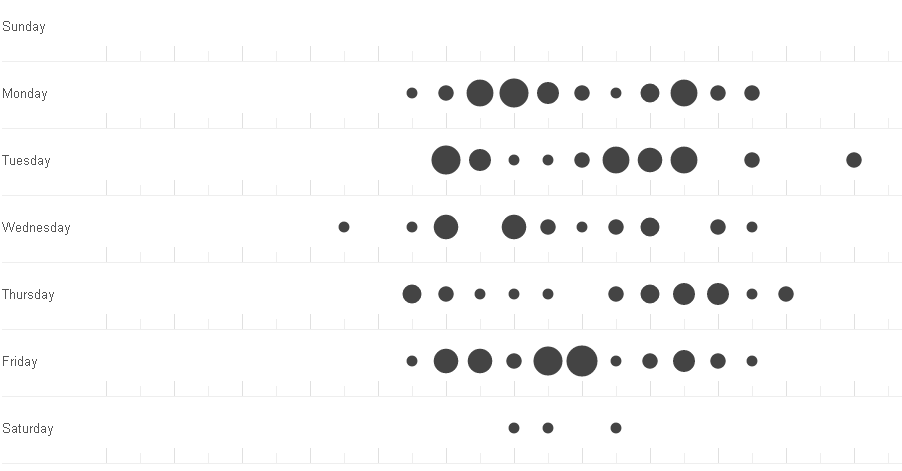
\includegraphics[width=15cm]{git.png}
\end{center}
\caption{GitHub Visualisation of Commits/Day}
\label{fig:git}
\end{figure}

\subsection{Integrated Development Environment}

The IDE used for this project was Spring Tool Suite [STS], a modified version of the open source IDE, Eclipse. The advantages of using STS over Eclipse are the pre configured services within the application. Tomcat, Maven, egit, and the core Spring dependencies themselves come pre-packaged within the application. Java EE and web application support are also present. One clear advantage of using STS over Eclipse is that if a organisation were using Eclipse as as IDE, they could be running a variety of different versions of application servers or plug ins. A pre-packaged solution like STS reduces the risks of bugs being introduced, or not being able to reproduce bugs, on different development environments.

\subsection{Logging}

Logging was used within the application to check both the flow of the application, as well as to pin point where certain lines of code were being called. The logging implementation used was log4j, an open source logging solution created by Apache. Log4j is designed with the possibility of enabling or disabling logging at run time. This is important in an application may have thousands of logging instances within it. This would be difficult to remove from production code, and would increase the risk of introducing bugs were it to be attempted. 

Logging can also be used to analyse usability and a "log will contain statistics about the frequency with which each user has used each feature in the program and the frequency with which various events of interest (such as error messages) have occurred." \parencite{holzinger2005usability}

\section{Usability Studies}

The criteria that govern usability were looked at within this project. In doing this, two other websites were examined: the current website for the club, and a site that was recommended to me by a club member, Tralee Tennis club. 

\subsection{Method of Evaluation}

The criteria for evaluating the websites in the case studies were adapted from \cite{smith2001applying}. Smith breaks down the criteria into two groups: \textit{Information Content Criteria} and \textit{Ease-of-use Criteria}. While accuracy of content is a factor in usability, it is outside the remit of a final year project. \textit{Ease-of-use Criteria} will be the sole group used for evaluation herein. 


\subsection{Case Study: Monaleen GAA Tennis Club}

The first site examined was the existing site for the club. This site is located at \newline\textit{http://www.monaleengaatennisclub.com/}. The current site is a basic HTML site with a CSS style sheet, that occasionally uses a PHP script to facilitate users to register for tournaments. It uses a basic architecture stack consisting of these HTML pages coupled with an Apache HTTP Server. The reasons for this choice that the club just needed a presence on the internet, there was no need for much functionality at the time, and simplicity.

This architectural choice places a number of constraints on the potential growth of the site however. The definition of roles within the system is not possible. An example would be that committee members cannot add news stories themselves, but must contain the web-master to perform this action on their behalf. There is also no scope to add secure features to the site, such as a members only feature. Any introduction of these features would require a considerable overhaul of the existing architecture.

The only NFR looked at during the development of the site was availability, which is fulfilled by the choice of architecture and lightweight implementation. 

\subsection{Case Study: Tralee Tennis Club}

The second site chosen as a comparison was the site for the Tralee Tennis Club. This site was mentioned during requirements elicitation, as members from Monaleen had travelled there for a tournament. While there was no opportunity to speak with the site administrator, the site has the appearance of a professional design. The site is developed with PHP and JavaScript. It facilitates the booking of available timetable slots through a user login system. This system is available through the website, and a physical kiosk on location. The type of web architecture, and the information pertaining to why these choices were made, were not available.  

The site is available at \textit{http://www.traleetennisclub.ie/}.

\section{Usability Results}
\label{sec:usabilty}

These criteria are based on a Yes-No answer. A Yes results in 1 point, where a No results in 0. Any exceptions are noted within the relevant tables.

\begin{table}[H]
\caption{Table 1 - Links}
\begin{center}
    \begin{tabular}{ | l | l | l | p{5cm} |}
    \hline
	\textbf{Criteria} & \textbf{Monaleen Tennis Club} & \textbf{Tralee Tennis Club}\\ \hline
	Links are updated? & No & Yes\\ \hline
	Short-cuts for frequent users? & No & No\\ \hline
	Warning if link leads to large file? & n/a & n/a\\ \hline
	Indication of restricted access for link & n/a & Yes\\ \hline
	Link text indicates nature of target & No & Yes\\ \hline
	Total & 0/5 & 3/5\\ \hline	
    \end{tabular}
\end{center}
\label{fig:table1}
\end{table}

\begin{table}[H]
\caption{Table 2 - Feedback Mechanisms}
\begin{center}
    \begin{tabular}{ | l | l | l | p{5cm} |}
    \hline
	\textbf{Criteria} & \textbf{Monaleen Tennis Club} & \textbf{Tralee Tennis Club}\\ \hline
	Contact Details for website maintainer & Yes & Yes\\ \hline
	Link to page maintainer on each page & Yes & Yes\\ \hline
	Forms provided for users to enter details & Yes* & No\\ \hline
	FAQ provided & No & Yes\\ \hline
	Feedback mechanisms are fully operational & No & No\\ \hline
	Total & 2.5/5 & 3/5\\ \hline	
    \end{tabular}
\end{center}
\label{fig:table2}
\end{table}
\textit{*Only when tournament sign ups are open, .5 mark as it is not a regular part of the site}

\begin{table}[H]
\caption{Table 3 - Accessability}
\begin{center}
    \begin{tabular}{ | l | l | l | p{5cm} |}
    \hline
	\textbf{Criteria} & \textbf{Monaleen Tennis Club} & \textbf{Tralee Tennis Club}\\ \hline
	Speed of site adequate& Yes & Yes\\ \hline
	Site Availability High?* & Yes & Yes\\ \hline
	Website made known through search tools** & .5/3 & 2.5/3\\ \hline
	Link back to parent entity & Yes & Yes\\ \hline	
	Name of entity reflected in URL & Yes & Yes\\ \hline	
	URL is not over complex,likely to be mistyped & No& No\\
	\hline	
	Total & 4.5/8 & 6.5/8\\ \hline	
    \end{tabular}
\end{center}
\label{fig:table3}
\end{table}
\textit{*While not possible to test extensively over a period of time, this write was never denied access at any time}\newline
\textit{**This was tested with 3 search engines: Google, Bing and Yahoo! Marked out of 3 - 1pt for first result, .5pt for first page, 0 for page 2+. Search terms were 'Limerick Tennis' and 'Kerry Tennis'}

\begin{table}[H]
\caption{Table 4 - Design}
\begin{center}
    \begin{tabular}{ | l | l | l | p{5cm} |}
    \hline
	\textbf{Criteria} & \textbf{Monaleen Tennis Club} & \textbf{Tralee Tennis Club}\\ \hline
	Format,Graphic Design Appropriate & Yes & Yes\\ \hline
	Pages appropriate length, clear, uncluttered& No & Yes\\ \hline
	Consistent format through website & No & Yes\\ \hline
	Site compatible with multiple browsers & Yes & Yes\\ \hline
	Site can be used without graphics & No & No\\ \hline
	Total & 2/5 & 4/5\\ \hline	
    \end{tabular}
\end{center}
\label{fig:table4}
\end{table}

\begin{table}[H]
\caption{Table 5 - Navigability}
\begin{center}
    \begin{tabular}{ | l | l | l | p{5cm} |}
    \hline
	\textbf{Criteria} & \textbf{Monaleen Tennis Club} & \textbf{Tralee Tennis Club}\\ \hline
	Website organised by anticipated user need & No & Yes\\ \hline
	Navigation options are distinct& Yes & Yes\\ \hline
	Conventional navigation models*& Yes & Yes\\ \hline
	Navigation links are provided on all pages & Yes & Yes\\ \hline
	Browsing facilitated by menu or site map &Yes & Yes\\ \hline
	Reach any point in appropriate number of clicks** & Yes & Yes\\ \hline
	Search Engine Provided & No & No\\ \hline
	Total & 5/7 & 6/7\\ \hline	
    \end{tabular}
\end{center}
\label{fig:table5}
\end{table}
\textit{*eg menu on top or left of screen}\newline
\textit{**defined as 3,} \cite{smith2001applying}

\begin{table}[H]
\caption{Table 6 - Results}
\begin{center}
    \begin{tabular}{ | l | l | p{5cm} |}
    \hline
	Site & Total\\ \hline
	Monaleen Tennis Club & 14/30\\ \hline
	Tralee Tennis Club & 22.5/30\\ \hline	
    \end{tabular}
\end{center}
\label{fig:table6}
\end{table}

Tralee Tennis Club is a clear winner with a site that adheres to the usability criteria defined by Smith. This site provides a benchmark in which to compare the application developed for this project.